\documentclass[english,brazilian]{UNISINOSmonografia}
\usepackage[utf8]{inputenc} % charset do texto (utf8, latin1, etc.)
\usepackage[T1]{fontenc} % encoding da fonte (afeta a sep. de sílabas)
\usepackage{graphicx} % comandos para gráficos e inclusão de figuras
\usepackage{bibentry} % para inserir refs. bib. no meio do texto

%=======================================================================
% Escolha do sistema para geração de referências bibliográficas.
%
% O default é usar o estilo unisinos.bst.  Comente a definição abaixo
% e descomente a linha seguinte para usar o estilo do ABNTeX (é
% necessário ter esse pacote instalado).
%
% A vantagem do unisinos.bst é que ele permite o uso de um arquivo .bib
% seguindo as orientações tradicionais do BibTeX (veja essas orientações
% em http://ctan.tug.org/tex-archive/biblio/bibtex/contrib/doc/btxdoc.pdf).
% Entretanto, o estilo não suporta algumas citações mais exóticas como
% apud.  Para isso, use o ABNTeX, mas esteja ciente de que muitas de
% suas referências serão incompatíveis com os estilos tradicionais do
% BibTeX como plain, alpha, ieeetr, entre outros.
%=======================================================================
\unisinosbst
%\usepackage[alf]{abntcite}

%=======================================================================
% Dados gerais sobre o trabalho.
%=======================================================================
\autor{Gräbin}{Paulo Henrique Grolli}
\titulo{Um modelo acessível de software para localização e navegação de deficiêntes visuais com Bluetooth Low Energy}
\orientador[Prof.~Dr.]{Costa}{Cristiano André da}
\local{São Leopoldo}
\ano{2015}

%% dados específicos para monografia de Graduação
\unidade{Unidade Acadêmica Graduação}
\curso{Curso de Bacharelado em Ciência da Computação}
\natureza{%
Trabalho de Conclusão de Curso apresentado como requisito parcial
para a obtenção do título de Bacharel em Ciência da Computação
pela Universidade do Vale do Rio dos Sinos --- UNISINOS
}

% cada palavra-chave deve ser fornecida duas vezes, uma em português e
% outra no idioma estrangeiro (na verdade, em tantos idiomas quantos se
% desejar).
\palavrachave{brazilian}{Acessibilidade Ubíqua}
\palavrachave{brazilian}{Deficiência Visual}
\palavrachave{brazilian}{Sistemas de Posicionamento Indoor}
\palavrachave{english}{Ubiquitous Accessibility}
\palavrachave{english}{Visual Impairment}
\palavrachave{english}{Indoor Positioning System}

%=======================================================================
% Início do documento.
%=======================================================================
\begin{document}
\capa
\folhaderosto
%\folhadeaprovacao % não deve ser incluída nos TCCs

%=======================================================================
% Dedicatória (opcional).
%
% O texto é normalmente colocado na parte de baixo da página, alinhado
% à direita.  Mas a formatação é basicamente livre.  Só não se escreve
% a palavra 'dedicatória'.
%=======================================================================
\begin{dedicatoria}
À minha meus pais que sempre me incentivaram na busca por conhecimento e a lutar pelos meus objetivos.\\[4ex] % quebra a linha dando um espaçamento maior


\begin{itshape} % faz o texto ficar em itálico
Learning is the only thing the mind never exhausts, \\
never fears, \\
and never regrets.\\
%If I have seen farther than others,\\
%it is because I stood on the shoulders of giants.\\
\end{itshape}
--- \textsc{Leonardo Da Vinci} % \textsc é o "small caps"
\end{dedicatoria}

%=======================================================================
% Agradecimentos (opcional).
%=======================================================================
\begin{agradecimentos}
Cristiano - orientador \\
Mãe pai e irmão \\
Namorada \\
Amigos \\
\end{agradecimentos}

%=======================================================================
% Epígrafe (opcional).
%
% ``[...] o autor apresenta uma citação, seguida de indicação de autoria,
% relacionada com a matéria tratada no corpo do trabalho. Podem, também,
% constar epígrafes nas folhas de aberturas das seções primárias.''
%=======================================================================
% \begin{epigrafe}
% ``\textit{Ninguém abre um livro sem que aprenda alguma coisa}''.\\
% (Anônimo)
% \end{epigrafe}

%=======================================================================
% Resumo em Português.
%
% A recomendação é para 150 a 500 palavras.
%=======================================================================
\begin{abstract}
O presente trabalho apresenta a modelagem de um sistema de posicionamento em ambientes internos, com recursos de acessibilidade, desenhado com o objetivo de ser usado por portadores de deficiência visual. O modelo consiste em uma aplicação a ser usada em dispositivos móveis, utilizando beacons transmissores Bluetooth espalhados pelo ambiente para obter a localização do usuário. Para permitir que seus usuários possam se deslocar em ambientes desconhecidos sem necessidade de auxilio de outras pessoas, o sistema objetiva fornecer uma localização confiavel e uma navegação segura e independente.
\end{abstract}

%=======================================================================
% Resumo em língua estrangeira (obrigatório somente para teses e
% dissertações).
%
% O idioma usado aqui deve necessariamente aparecer nos parâmetros do
% \documentclass, no início do documento.
%=======================================================================
\begin{otherlanguage}{english}
\begin{abstract}
This paper presents the modeling of a Indoor Positioning System with accessibility features, designed aiming to be used by visually impaired users. The model consists of an application to be used in mobile devices, making use of Bluetooth beacons deployed in the environment to obtain users location. In order to allow the users to navigate in unknown environments without need of assistance of other people, the system aims to provide a realiable location and a safe and independent navigation.
\end{abstract}
\end{otherlanguage}

%=======================================================================
% Lista de Figuras (opcional).
%=======================================================================
\listoffigures

%=======================================================================
% Lista de Tabelas (opcional).
%=======================================================================
\listoftables

%=======================================================================
% Lista de Abreviaturas (opcional).
%
% Deve ser passada como parâmetro a maior das abreviaturas utilizadas.
%=======================================================================
% \begin{listadeabreviaturas}{seg., segs.}
% \item[ampl.] ampliado, -a
% \item[atual.] atualizado, -a
% \item[coord.] coordenador
% \item[N.~T.] Novo Testamento
% \item[seg., segs.] seguinte, -s
% \end{listadeabreviaturas}

%=======================================================================
% Lista de Siglas (opcional).
%
% Deve ser passada como parâmetro a maior das siglas utilizadas.
%=======================================================================
\begin{listadesiglas}{FAPERGS}
\item[API] Application Programming Interface
\item[BLE] Bluetooth Low Energy
\item[GPS] Global Positioning System
\item[HTTP] Hypertext Transfer Protocol
\item[IBGE] Instituto Brasileiro de Geografia e Estatística
\item[JSON] JavaScript Object Notation
\item[NFC] Near Field Communication
\item[PDV] Portadores de Deficiência Visual
\item[RFID] Radio Frequency Identification
\item[SDK] Software Development Kid
\item[SIG] Special Interest Group
\item[SOAP] Simple Object Access Protocol
\item[TAM] Technology Acceptance Model
\item[UML] Unified Modeling Language
\item[XML] Extensible Markup Language
\end{listadesiglas}

%=======================================================================
% Lista de Símbolos (opcional).
%
% Deve ser passado o maior (mais largo) dos símbolos utilizados.
%=======================================================================
%\begin{listadesimbolos}{Ca}
%\item[\textsuperscript{o}C] Graus Celsius
%\item[Al] Alumínio
%\item[Ca] Cálcio
%\end{listadesimbolos}

%=======================================================================
% Sumário
%=======================================================================
\tableofcontents

%=======================================================================
% Introdução
%=======================================================================
\chapter{Introdução}
\epigrafecap{Eureka}{EINSTEIN, Albert}

	\section{Motivação}

	\section{Objetivos}
	
		\subsection{Objetivo geral}
		
		\subsection{Objetivos específicos}
	
	\section{Estrutura do Texto}

%=======================================================================
% Referencial Teórico
%=======================================================================
\chapter{Referencial Teórico}

	\section{Deficiência Visual}
De acordo com o levantado por \citetexto{IBGE2010} no último Censo Demográfico, realizado em 2010, o Brasil possuia 45,6 milhões de pessoas que afirmaram ser portadoras de deficiência. Desse total, 35,7 milhões, ou 78,2\%, são portadores de deficiência visual (PDV).

A deficiência visual impõe severas dificuldades em todos os aspectos da vida dos que são afetados por ela, dificultando diversos aspectos de sua vida, como o seu deslocamento em ambientes desconhecidos. Não é possível compreender a dificuldade que um cego possui em realizar as tarefas consideradas triviais por aqueles que possuem a totalidade de sua visão.

No Brasil, existe legislação especifica para tratar da condição médica necessária para classificar alguém como deficiente visual e, também, para garantir a acessibilidade e os direitos dos PDV. Os Decretos 3.298/99 e 5.296/04 definem critérios técnicos para conceituação de alguém como PDV. Os níveis de deficiência visual são baixa visão e cegueira, baseados na acuidade visual medida através de exame. A Lei 10.098/00 estabelece normas e critérios básicos para a promoção da acessibilidade, descrevendo normas de construção de edifícios públicos, de uso coletivo e privados, bem como regulando como deve se dar a acessibilidade nos sistemas de comunicação e sinalização.
	
	\section{Computação Móvel e Ubíqua}
Tecnologias tão avançadas que deixam de ser um fim em si mesmas e passam a ser um meio para que as pessoas realizem seus afazeres. Tão conectados, tão presentes na nossa rotina e concebidas para naturalmente se integrarem em nossas vidas que deixam de ser percebidas e se colocam no plano de fundo da nossa percepção. É assim que Weiser (1991) começa introduzindo o conceito de computação ubíqua. 

Weiser previu um mundo onde computadores deixariam de possuir apenas o tamanho de um notebook que é usado em cima de uma mesa. Um mundo onde computadores seriam pequenos o suficiente para serem embutidos em botões de uma camisa e também grandes o suficiente para ocuparem os ambientes em que convivemos, estudamos ou trabalhamos. Esses computadores conversariam entre si de maneira continua e transparente, de modo que eles e todos os usuários estariam permanentemente conectados entre si, permitindo que serviços estejam acessíveis em todos os lugares e em todos os momentos. Tal definição vai ao encontro do conceito estabelecido por Satyanarayanan (2011) para computação móvel como sendo: “Informação na ponta dos dedos em qualquer lugar e em qualquer tempo”.
	
	\section{Tecnologias Assistivas}
Diversas ferramentas existem para promover a inclusão de PDV, bem como para aliviar as dificuldades impostas pela deficiência visual. Cães-guia, bengalas e piso tátil são as principais formas usadas pra facilitar locomoção.

Ganz et al. (2014) destaca que smartphones são ferramentas extremamente benéficas no dia a dia das PDV, podendo ser utilizados em diversas finalidade, tais como reconhecimento de cédulas de dinheiro, objetos e cores, navegação na internet, leitura de e-mails e comunicação. O trabalho ainda afirma que o uso de smartphones é possível devido à presença de recursos de acessibilidade oferecidos pelos principais sistemas operacionais disponíveis. 

Entre esses recursos, podemos destacar a leitura de telas e os alertas vibratórios, essenciais pra aqueles que não enxergam as telas sensíveis ao toque que equipam a grande maioria dos smartphones disponíveis atualmente. Ao invés de apenas ler o texto sendo exibido, essa funcionalidade também informa sobre os tipos de cada componente, possibilitando ao usuário saber como lidar com cada um.

Mau et al. (2008), após pesquisa realizada em seu trabalho, define o telefone celular como “a peça de tecnologia mais valiosa para os cegos”. 

Segundo o estudo realizado por Quinõnes et al. (2011), PDV possuem o desejo de carregar consigo a menor quantidade possível de equipamento. É necessário criar tecnologias que não sejam um fardo a ser carregado, mas que ofereçam a quantidade apropriada de informações ao usuário. Uma maneira citada pelo autor é a incorporação de tecnologias de navegação em aparelhos que deficientes visuais carreguem consigo normalmente, assim reduzindo o número de objetos que devem ser cuidados.
	
	\section{Sistemas de localização}
Bluetooth é uma tecnologia de comunicação sem fios de curto alcance, lançada comercialmente em 1990, quando teve sua primeira especificação formal divulgada. Desde então diversas modificações foram feitas e a tecnologia passou por diversos aprimoramentos, estando atualmente na versão 4.x, também conhecida como Bluetooth Smart, lançada em 2010. 

O Bluetooth foi criado e atualmente é mantido por um conjunto de empresas conhecido como Bluetooth Special Interest Group (SIG). Inicialmente formado por Ericsson, Intel, Nokia, Toshiba e IBM, o SIG é hoje composto por mais de 20.000 empresas, incluindo Apple, Microsoft, Motorola e Lenovo.

A tecnologia possui duas formas distintas de atuação, apesar de compartilharem entre si alguns pontos em comum. O primeiro e mais antigo modo, disponível desde a primeira especificação, é chamado Basic Rate (BR). O segundo foi introduzido somente na versão 4.0 e é chamado Low Energy (LE) e é o modo que será utilizado pelo modelo que será proposto.

O LE foi criado para permitir produtos que requerem baixíssimo consumo de energia e baixo custo, quando comparados ao outro modo. Assim sendo, esse modo foi pensado para aplicações que exigem pouca troca de informações. Um exemplo de produto viável com a chegada do modo LE são os beacons bluetooth, que consistem em dispositivos do tamanho de uma moeda comum, compostos por um processador, uma bateria e um transmissor, que transmitem informações sobre si em intervalos regulares. Como o sinal dos beacons tem seu alcance limitado a alguns poucos metros, foi introduzido o conceito de micro localização, tornando possível o desenvolvimento de aplicações novas aplicações e serviços onde antes não era possível, tais como lojas e pontos de venda, grandes shows ou eventos, estádios esportivos, localização em ambientes internos, etc.

A imensa maioria dos telefones celulares hoje fazem uso nativo da tecnologia, não exigindo qualquer tipo de equipamento adicional.

Taylor et al. (2012) revelam que diversas tecnologias foram utilizadas anteriormente em modelos de sistema para navegação para PDV. Sonares, Radio Frequency Identification (RFID), Near Field Communication (NFC), bluetooth e Global Positioning System (GPS) são algumas dessas tecnologias. Os autores ainda apontam que apesar de todas elas oferecerem vantagens em suas propostas, todas também possuem pontos fracos:

\begin{itemize}
  \item GPS é normalmente usado para localização em ambientes externos, mas se mostra ineficiente devido à própria natureza das ondas de rádio usadas na tecnologia, quando obstáculos são locados ao redor do usuário. Além disso, GPS não é uma tecnologia ideal para ambientes internos, pois é capaz apenas de marcar um ponto em um mapa, não sendo suficiente para indicar, por exemplo, múltiplos andares em um prédio, cenário muito comum em ambientes indoor. 
  \item Sonares são formas baratas de detecção de objetos e obstáculos, através de frequências acústicas, mas exigem hardware dedicado e não servem para localização.
  \item RFID, juntamente com NFC, exige proximidade de seus emissores para que a comunicação seja estabelecida.
  \item Os autores não chegam a citar nominalmente os pontos fracos da tecnologia bluetooth, mas um grande ponto que pode ser citado é o consumo de bateria causado pelas versões que antecederam a versão 4, também chamada de bluetooth low energy.    \ldots
\end{itemize}

%=======================================================================
% Trabalhos relacionados
%=======================================================================
\chapter{Trabalhos Relacionados}

	\section{Trabalho 1}
	
	\section{Trabalho 2}

	\section{Trabalho 3}
	
	\section{Comparação entre os trabalhos estudados}

%=======================================================================
% Modelo proposto
%=======================================================================
\chapter{Modelo Proposto}
Visando mitigar o impacto da deficiência visual na vida dos usuários, o modelo proposto fará uso de dispositivos móveis aliados aos conceitos da computação ubíqua para auxiliar os PDV durante o deslocamento em ambientes internos, tais como o campus da Unisinos, através de instruções dadas por voz e alertas vibratórios. O modelo oferecerá as funcionalidades de informar a localização atual, pesquisar locais, mostrar locais de conveniência (restaurantes, agências bancárias, etc), informar rota mais curta até o local selecionado e salvar local como favorito, entre outras. Para as funcionalidades espaciais, o modelo usará beacons transmissores bluetooth previamente espalhados pelo campus.

O modelo objetiva oferecer localização confiável a seus usuários através de seus smartphones sem necessidade de hardware dedicado, assim possibilitando navegação segura e independente, tendo baixo custo e facilidade de implantação.

	\section{Requisitos}
	
	\section{Arquitetura}

%=======================================================================
% Metodologia
%=======================================================================
\chapter{Metodologia}
Quanto à natureza da pesquisa, esse trabalho ceracteriza-se como uma pesquisa aplicada, pois objetiva gerar conhecimento 

	\section{Desenvolvimento}
	
	\section{Avaliação}


\chapter{Conclusão}

	\section{Comparação entre os trabalhos estudados e o modelo proposto}
	
	\section{Trabalhos futuros}








\chapter{Introdução}

% as epígrafes nos capítulos são opcionais
\epigrafecap{The reasonable man adapts himself to the world; the unreasonable one persists in trying to adapt the world to himself. Therefore all progress depends on the unreasonable man.}{George Bernard Shaw}

Conforme \citetexto{Hexsel11}, a introdução tem o objetivo de ``\emph{introduzir} o material que vai ser apresentado em mais detalhe nas seções subseqüentes''. Na introdução você deve contextualizar o problema e mostrar por que vale a pena resolvê-lo. Você deve apresentar a solução proposta e mostrar o seu diferencial em relação aos trabalhos relacionados. Observe, porém, que na introdução você deve apenas tratar do O QUÊ e PORQUÊ, sem tratar do como \cite{Hexsel11}, que deve ser explicado na seção que descreve o trabalho desenvolvido.

Geralmente, a introdução tem uma estrutura similar ao resumo e deve apresentar:
\begin{itemize}
	\item \textbf{Contexto e motivação:} Aqui você deve apresentar o contexto do trabalho (área de que ele se trata) e uma motivação para trabalhar nesse assunto.
	\item \textbf{Problema:} Aqui você vai apresentar um problema, uma lacuna, observada na área e que você pretende tratar. Você deve se perguntar aqui: ``Que respostas estou disposto a responder?''. O problema deve ser definido claramente e delimitado em termos de espaço de tempo. Veja que essa parte visa alertar o leitor de que o que você está propondo é uma solução para um problema observado na área. 
	\item \textbf{Objetivos:} Aqui você deve apresentar os objetivos do seu trabalho. Tome cuidado para não confundir objetivos com atividades.   Faça a si mesmo a pergunta: ``O que pretendo alcançar com a pesquisa?''. Você pode discernir entre objetivos gerais e objetivos específicos:
	\begin{itemize}
		\item Objetivo geral --- qual o propósito da pesquisa?
		\item Objetivos específicos --- abertura do objetivo geral em outros menores (possíveis capítulos).
	\end{itemize}
	Veja abaixo um exemplo de objetivo retirado da monografia de~\citetexto{Teixeira09}:

	Com a possibilidade de acesso a base de dados XML gerada a partir do Sistema de Currículos Lattes e a necessidade de melhor reutilizar as informações existentes neste sistema, o presente trabalho tem como objetivo geral permitir o acesso do pesquisador a seus dados através de uma interface mais amigável: o padrão LaTeX. Para isto destacam-se os seguintes objetivos específicos:
	\begin{alineas}
		\item identificar e analisar o formato de especificação de currículos da Plataforma Lattes;
		\item disponibilizar uma ferramenta para a geração de uma representação de dados intermediária a partir do formato especificado;
		\item implementar a tradução dos dados colhidos em código LaTeX através da utilização da ferramenta criada;
		\item analisar os resultados obtidos e as alternativas presentes no uso da ferramenta.
	\end{alineas}
\end{itemize}

%=======================================================================
% Escrevendo o Texto
%=======================================================================
\chapter{Escrevendo o Texto}

\section{Comandos do \LaTeX}
Como regra geral, use os comandos tradicionais do \LaTeX\ para formatar seu texto.  Neste documento procuramos demonstrar os comandos mais comumente utilizados em monografias acadêmicas.

Neste capítulo apresentamos alguns exemplos de como colocar figuras e tabelas no seu texto.

\section{Ilustrações}

\subsection{Legendas}
As legendas das figuras devem se encontrar no topo da figura e não abaixo, como usualmente colocado. Abaixo da figura, é obrigatório colocar a fonte (mesmo que a figura tenha sido do próprio autor).

As legendas devem conter o tipo da ilustração (Figura, Tabela, etc), seguido de numeração simples (sem número do capítulo).

Toda figura deve ser citada no texto, como nos exemplos que seguem.

\subsection{Figuras}
A Figura~\ref{fig:escrita} ilustra as fases psicológicas da escrita da dissertação. Você vai se reconhecer no personagem. ;-)

\begin{figure}
	\caption{Fases psicológicas da escrita da dissertação}
	\label{fig:escrita}
	\centering%
	\begin{minipage}{.8\textwidth}
		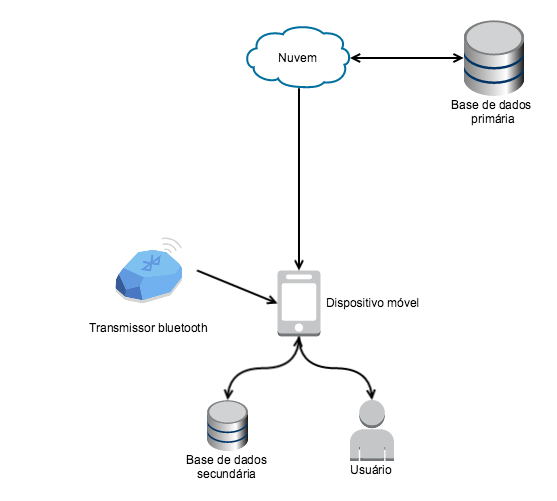
\includegraphics[width=\textwidth]{escrita}
		\fonte{\citetexto{Cham12}}
	\end{minipage}
\end{figure}

\subsection{Tabelas}
A Tabela~\ref{tab:estacoes} é um exemplo de tabela elaborada pelo(a) próprio(a) autor(a).

\begin{table}
	\caption{Período das estações do ano no Brasil}
	\label{tab:estacoes}
	\centering%
	\begin{minipage}{.6\textwidth}
		\begin{tabular*}{\textwidth}{ll}
			\hline
			\textbf{Meses} & \textbf{Estações do Ano}\\
			\hline
			21 de março a 21 de junho & Outono\\
			21 de junho a 23 de setembro & Inverno\\
			23 de setembro a 21 de dezembro & Primavera\\
			21 de dezembro a 21 de março & Verão\\
			\hline
		\end{tabular*}
		\fonte{Elaborada pela autora.}
	\end{minipage}
\end{table}

\section{Resumo}
O resumo deve conter de 100 a 500 palavras. No resumo não deve haver citações e indica-se que essa seja a última seção do texto a ser escrita. Veja abaixo uma sugestão de organização e exemplo de resumo de \citetexto{Moro11}.

Sugestão (uma a três linhas para cada item):
\begin{itemize}
	\item Contexto geral e específico;
	\item Questão/problema sendo investigado (propósito do trabalho);
	\item Estado-da-arte (por que precisa de uma solução nova/melhor);
	\item Solução (nome da proposta, metodologia básica sem detalhes, quais características respondem as questões iniciais, interpretação dos resultados, conclusões).
\end{itemize}

Exemplo (SANTOS et al., 2008 apud \citealp{Moro11}):
\begin{quote}
CONTEXTO: A Web é abundante em páginas que armazenam  dados de forma implícita. PROBLEMA: Em muitos casos, estes dados estão presentes em textos semiestruturados sem a presença de delimitadores explícitos e organizados em uma estrutura também implícita. SOLUÇÃO: Este artigo apresenta uma nova abordagem para extração em textos semi-estruturados baseada em Modelos de Markov Ocultos (Hidden Markov Models - HMM). ESTADO-DA-ARTE e MÉTODO PROPOSTO: Ao contrário de outros trabalhos baseados em HMM, a abordagem proposta dá ênfase à extração de metadados, além dos dados propriamente ditos. Esta abordagem consiste no uso de uma estrutura aninhada de HMMs, onde um HMM principal identifica os atributos no texto e HMMs internos, um para cada atributo, identificam os dados e metadados. Os HMMs são gerados a partir de um treinamento com uma fração de amostras da base a ser extraída. RESULTADOS: Os experimentos realizados com anúncios de classificados retirados da Web mostram que o processo de extração alcança qualidade acima de 0,97 com a medida F, mesmo se esta fração de treinamento é pequena. 
\end{quote}

%=======================================================================
% Exemplos de Citações e Referências Bibliográficas
%=======================================================================
\chapter{Exemplos de Citações e Referências Bibliográficas}
\nobibliography* % para usar o \bibentry
Neste capítulo são apresentados exemplos de citações e referências bibliográficas.  Aqui é utilizado o pacote \texttt{bibentry}, que permite a inserção de referências no meio do texto (atenção para a diferença entre citações e referências).

Você vai ver que, neste exemplo, não está sendo usado o estilo de referências bibliográficas do projeto ABNTeX\footnote{http://http://sourceforge.net/projects/abntex}.  Você é completamente livre para usá-lo (veja no início do arquivo .tex como fazer isso).  Os motivos para não usar o ABNTeX neste exemplo são basicamente dois:
\begin{itemize}
	\item Para usar o ABNTeX, é necessário instalá-lo em seu sistema \TeX\ primeiro; embora não seja uma tarefa tão complicada, enxergamos como uma dificuldade a mais para o usuário iniciante.  Nosso objetivo aqui é facilitar ao aluno da UNISINOS o uso deste modelo, de modo que basta copiar os arquivos \texttt{UNISINOSmonografia.cls} e \texttt{unisinos.bst} para a pasta onde estão seus arquivos .tex;
	\item As normas da ABNT são tão complexas que, para atender a todas as variações possíveis de citações e referências, o projeto ABNTeX criou uma série de campos adicionais nas entradas do arquivo .bib.  Embora funcione para o caso ABNT, o efeito colateral de fazer isso é que o seu arquivo .bib será muitas vezes incompatível com os demais estilos tradicionais do BibTeX, como \texttt{plain}, \texttt{alpha}, \texttt{ieeetr}, entre outros.  Por exemplo, em referências a artigos publicados em conferências, o campo \texttt{organization} é usado pelo ABNTeX para definir o nome do evento.  Isso não é padrão e não será reconhecido pelos estilos tradicionais\footnote{Veja como criar seus arquivos .bib no manual do BibTeX, que pode ser encontrado em http://ctan.tug.org/tex-archive/biblio/bibtex/contrib/doc/btxdoc.pdf.}.  Considerando que um dos maiores benefícios do BibTeX é criar um arquivo .bib que pode ser reutilizado pelo resto da vida, nossa estratégia com o \texttt{unisinos.bst} foi tentar aproximar ao máximo a formatação exigida pela ABNT sem implicar na criação de arquivos .bib incompatíveis.  Isso funciona bem na grande maioria dos casos, mas não em todos.  Nesse caso, a saída é usar o ABNTeX ou então alterar manualmente o arquivo .bbl que é gerado ao rodar o comando \texttt{bibtex}.
\end{itemize}

Em caso de dúvida, siga as orientações do manual da Biblioteca \cite{Biblioteca11} e, se necessário, da norma NBR~6023 \cite{NBR6023:2002}.

\section{Citações}
As citações podem ocorrer de duas formas: com os nomes dos autores inseridos no texto ou não.  Isso implica em uma construção diferente para as frases.  Por exemplo:
\begin{itemize}
	\item Com o nome do autor inserido no texto: ``De acordo com \citetexto{Tanenbaum03}, o modelo de referência OSI foi proposto de forma tardia.''
	\item Sem inserir o autor no texto: ``O modelo de referência OSI foi proposto de forma tardia \cite{Tanenbaum03}.''
\end{itemize}

\section{Livros}
Seguem alguns exemplos de referências de livros:
\begin{itemize}
	\item \bibentry{Buford09}.
	\item Livro com indicação de edição:\\
	\bibentry{Kurose10ptbr}.
\end{itemize}

\section{Artigos em Periódicos}
Os exemplos abaixo ilustram referências a artigos em periódicos.
\begin{itemize}
	\item \bibentry{Hayes08}.
	\item \bibentry{Lawton08}.
\end{itemize}

\section{Artigos em Conferências}
\begin{itemize}
	\item \bibentry{Laadan10}.
	\item \bibentry{Anderson95}.
\end{itemize}

\section{Teses e Dissertações}
Seguem algumas referências a trabalhos acadêmicos, como teses, dissertações, trabalhos de conclusão de curso, etc.
\begin{itemize}
	\item \bibentry{Teixeira09}.
	\item \bibentry{Flaumann05}.
\end{itemize}

%=======================================================================
% Referências
%=======================================================================
\bibliography{exemplo}

%=======================================================================
% Exemplo de Apêndice
% O Apêndice é utilizado para apresentar material complementar elaborado
% pelo próprio autor.  Deve seguir as mesmas regras de formatação do
% corpo principal do documento.
%=======================================================================
% \appendix
% \chapter{Informações Complementares}

% O Apêndice é o lugar para incluir textos complementares, que não são essenciais para o entendimento do assunto principal da monografia, mas que podem contribuir com informação relevante (por exemplo, uma prova matemática, uma conceituação básica, etc.).  Ele deve seguir o formato normal do documento.

%=======================================================================
% Exemplo de Anexo
% O Anexo é utilizado para a ``inclusão de materiais não elaborados pelo
% próprio autor, como cópias de artigos, manuais, folders, balancetes, etc.
% e não precisam estar em conformidade com o modelo''.
%=======================================================================
% \annex
% \chapter{Artigos Publicados}
% Existe diferença entre os Apêndices e os Anexos.  Os apêndices trazem informação escrita pelo próprio autor do trabalho, incorporando-se ao formato da monografia como um todo.  Já um anexo é um material à parte, definido/publicado por si só, e que o autor julga conveniente ser apresentado juntamente com a monografia.  Normalmente também vai apresentar formato próprio, como um artigo publicado, um folder, uma planilha, etc.
\end{document}